\documentclass[12pt,a4paper]{article}

% Language and formatting
\usepackage{polyglossia}
\usepackage{csquotes} %fvextra to avoid warning?
\setmainlanguage[variant=brazilian]{portuguese}

% \usepackage[backend=biber, style=alphabetic, sorting=ynt]{biblatex}
% \addbibresource{bibliography.bib}

% \setmainfont{Palatino Linotype}
% \setmathfont{Palatino Linotype}
\usepackage[a4paper, margin=1.5cm]{geometry}
\usepackage{booktabs}

% % title header
% \usepackage{titleps}% http://ctan.org/pkg/titleps
% \makeatletter
% \newpagestyle{main}{% Define page style main
%     \sethead%
%     [\textbf\thepage][][\thechapter.\ \chaptertitle]% [<even-left>][<even-center>][<even-right>]
%     {\thesection.\ \sectiontitle}{}{\textbf\thepage}% {<odd-left>}{<odd-center>}{<odd-right>}
%     \setfoot{}{}{}% {<left>}{<center>}{<right>}
% }
% \pagestyle{main}% Use page style main

% Images
\usepackage{tikz}
\usetikzlibrary{cd}
\usepackage{graphicx, caption, subcaption}
\usepackage{float}

% Math tools
\usepackage{amsfonts, mathtools, amssymb, amsmath, amsthm, enumitem}
\usepackage{newpxtext, newpxmath}
\numberwithin{equation}{section}
\usepackage[ISO]{diffcoeff}
\usepackage{tensor}
\usepackage{siunitx}

% Misc
\usepackage{luacolor}
\usepackage[breakable]{tcolorbox}

\difdef{fp}{}{
    outer-Ldelim = \left.,
    outer-Rdelim = \right|,
    sub-nudge=0 mu
}
\newcommand\todo[1][!]{{\color{Red} TODO {#1}}}
\difdef{l}{i}{outer-Rdelim = \,, outer-Ldelim=}
\NewDocumentCommand\dli{}{\dl.i.}
\DeclareMathOperator\Riem{Riem}
\DeclareMathOperator\Orb{Orb}
\DeclareMathOperator\Stab{Stab}
\DeclareMathOperator\sgn{sgn}
\DeclareMathOperator\End{End}
\DeclareMathOperator\tr{tr}
\DeclareMathOperator\sech{sech}
\DeclareMathOperator\hor{hor}
\DeclareMathOperator\ver{ver}
\DeclarePairedDelimiter\abs{\lvert}{\rvert}
\DeclarePairedDelimiter\norm{\lVert}{\rVert}
\DeclarePairedDelimiterX\inner[2]{\langle}{\rangle}{#1,\mathopen{}#2}
\DeclarePairedDelimiter\set{\{}{\}}

\newenvironment{smallpmatrix}{\left(\begin{smallmatrix}}{\end{smallmatrix}\right)}
\newcommand\ract{\mathbin{\vartriangleleft}}
\newcommand\ractalt{\mathbin{\blacktriangleleft}}
\newcommand\lact{\mathbin{\vartriangleright}}
\newcommand\lactalt{\mathbin{\blacktriangleright}}
\newcommand\ad[1]{\operatorname{ad}_{#1}}
\newcommand\Ad[1]{\operatorname{Ad}_{#1}}
\newcommand\preim[2]{\operatorname{preim}_{#1}{\left(#2\right)}}
\newcommand\id[1]{\operatorname{id}_{#1}}
\newcommand\colorunderline[2]{{\color{#1}\underline{{\color{black}{#2}}}}}
\newcommand\Hom[2][]{\ensuremath{\operatorname{Hom}_{#1}{\left(#2\right)}}}
\newcommand\bundle[3]{\ensuremath{#1 \mathrel{\overset{#2}{\to}} #3}}
\newcommand\smooth[1]{\ensuremath{\mathcal{C}^\infty(#1)}}
\newcommand\sections[1]{\ensuremath{\Gamma\left(#1\right)}}
\newcommand\forms[2][]{\ensuremath{\Lambda^{#1}{\left({#2}\right)}}}
\newcommand\ffamily[3]{\ensuremath{\set*{#1}_{#2}^{#3}}}
\newcommand\family[2]{\ensuremath{\set*{#1}_{#2}}}
\newcommand\vetor[1]{\ensuremath{\boldsymbol{#1}}}
\newcommand\linear{\ensuremath{\mathrel{\tilde{\to}}}}
\newcommand\topology[1]{\ensuremath{\left(#1, \mathcal{O}_{#1}\right)}}
\newcommand\manifold[1]{\ensuremath{\left(#1, \mathcal{O}_{#1}, \mathscr{A}_{#1}\right)}}
\newcommand\restrict[2]{\ensuremath{\left.#1\right\rvert_{#2}}}
\newcommand\bfield[1]{\ensuremath{\diffp*{}{#1}}}
\newcommand\bvec[3][]{\ensuremath{\diffp*{#1}{#2}[#3]}}
\newcommand\bset[3]{\ensuremath{\set*{\diffp*{}{{#1}^1}[#3], \dots, \diffp*{}{{#1}^{#2}}[#3]}}}
\newcommand\pf[2][]{\ensuremath{{#2}_{\ast{#1}}}}
\newcommand\pb[2][]{\ensuremath{{#2}^{\ast}_{#1}}}

% catppuccin (latte)
\definecolor{Rosewater}{RGB}{220,138,120}
\definecolor{Flamingo}{RGB}{221,120,120}
\definecolor{Pink}{RGB}{234,118,203}
\definecolor{Mauve}{RGB}{136,57,239}
\definecolor{Red}{RGB}{210,15,57}
\definecolor{Maroon}{RGB}{230,69,83}
\definecolor{Peach}{RGB}{254,100,11}
\definecolor{Yellow}{RGB}{223,142,29}
\definecolor{Green}{RGB}{64,160,43}
\definecolor{Teal}{RGB}{23,146,153}
\definecolor{Sky}{RGB}{4,165,229}
\definecolor{Sapphire}{RGB}{32,159,181}
\definecolor{Blue}{RGB}{30,102,245}
\definecolor{Lavender}{RGB}{114,135,253}
\definecolor{Text}{RGB}{76,79,105}
\definecolor{Subtext1}{RGB}{92,95,119}
\definecolor{Subtext0}{RGB}{108,111,133}
\definecolor{Overlay2}{RGB}{124,127,147}
\definecolor{Overlay1}{RGB}{140,143,161}
\definecolor{Overlay0}{RGB}{156,160,176}
\definecolor{Surface2}{RGB}{172,176,190}
\definecolor{Surface1}{RGB}{188,192,204}
\definecolor{Surface0}{RGB}{204,208,218}
\definecolor{Base}{RGB}{239,241,245}
\definecolor{Mantle}{RGB}{230,233,239}
\definecolor{Crust}{RGB}{220,224,232}

% References
\usepackage{hyperref}
\usepackage[brazilian,capitalize,nameinlink,noabbrev]{cleveref}
\makeatletter
\hypersetup{
    pdftitle=\@title,
    pdfauthor=\@author,
    colorlinks=true,
    linkcolor=Mauve,
    citecolor=pink,
    filecolor=red,
    urlcolor=blue,
    bookmarksdepth=4
}
\makeatother

% tcolorbox environments
\tcbuselibrary{theorems}
% theorem
\newtcbtheorem[auto counter, crefname={Teorema}{Teoremas}]{theorem}{Teorema}%
{breakable,colback=Mauve!5,colframe=Mauve!95!black,fonttitle=\bfseries}{thm}

% definition
\newtcbtheorem[auto counter, crefname={Definição}{Definições}]{definition}{Definição}%
{breakable, colback=Pink!5,colframe=Pink!95!black,fonttitle=\bfseries}{def}

% proposition
\newtcbtheorem[auto counter, crefname={Proposição}{Proposições}]{proposition}{Proposição}%
{breakable,colback=Lavender!5,colframe=Lavender!95!black,fonttitle=\bfseries}{prop}

% lemma
\newtcbtheorem[auto counter, crefname={Lema}{Lemas}]{lemma}{Lema}%
{breakable,colback=Flamingo!5,colframe=Flamingo!95!black,fonttitle=\bfseries}{lem}

\title{4300337 - Lista de exercícios 1}
\author{Louis Bergamo Radial}

\begin{document}
\maketitle
\section*{Exercício 1}
No referencial \(K\), a partícula se move com velocidade \(v = 0.998c\) em direção ao chão. Assim, se a produção do múon ocorre à altitude \(h \approx \SI{15}{\kilo\meter}\), então o tempo \(t\) transcorrido desde o tempo de produção até a chegada da partícula no chão é
\begin{equation*}
    t = \frac{h}{v} \approx \SI{5.0e-5}{\second}.
\end{equation*}
Se \(\tau' = \SI{2.2e-6}{\second}\) é a vida média no referencial \(K'\) de repouso do múon, então no referencial \(K\), a vida média é
\begin{equation*}
    \tau = \gamma(v)\tau' = \SI{3.5e-5}{\second},
\end{equation*}
em que \(\gamma(v) = \left[1 - \left(\frac{v}{c}\right)^2\right]^{-\frac12}\).
Assim, a probabilidade da detecção de um múon no chão neste referencial é
\begin{equation*}
    p = \exp{\left(-\frac{t}{\tau}\right)} \approx 0.24.
\end{equation*}

No referencial \(K'\), o chão se move em direção à partícula com velocidade \(v\). Pela contração de Lorentz, se a distância percorrida no referencial \(K\) é \(h\), no referencial \(K'\) o chão se move uma distância \(h'\) dada por
\begin{equation*}
    h' = \frac{h}{\gamma(v)} \approx \SI{0.95}{\kilo\meter}.
\end{equation*}
Dessa forma, o tempo \(t'\) transcorrido desde a produção do múon e a chegada do chão ao múon é
\begin{equation*}
    t' = \frac{h'}{v} \approx \SI{3.2e-6}{\second}.
\end{equation*}
Assim, a probabilidade da detecção de um múon no chão neste referencial é
\begin{equation*}
    p' = \exp{\left(-\frac{t'}{\tau'}\right)} \approx 0.24,
\end{equation*}
o mesmo valor obtido no referencial \(K\).

\section*{Exercício 2}
Sejam \(t_1\) o instante em que o jato é emitido e \(t_2 = t_1 + \Delta t\) um instante posterior. Nestes instantes, sinais luminosos são emitidos em direção ao observador em \(O\), que os recebe nos instantes \(t_1' = t_1 + \frac{r + v\Delta t \cos\theta}{c}\) e \(t_2' = t_2 + \frac{r}{c}\). Deste modo, os sinais são recebidos em \(O\) em um intervalo \(\Delta t' = t_2' - t_1'\) dado por
\begin{equation*}
    \Delta t' = \Delta t \left(1 - \beta\cos\theta\right),
\end{equation*}
em que \(\beta = \frac{v}{c}\). A distância percorrida entre as emissões dos sinais luminosos é \(v\Delta t \sin\theta,\) de modo que a velocidade aparente \(v_{\mathrm{ap}} = \frac{v \Delta t \sin\theta}{\Delta t'}\) medida em \(O\) é
\begin{equation*}
    v_{\mathrm{ap}} = \frac{\beta \sin \theta}{1 - \beta \cos \theta}c.
\end{equation*}

O ângulo \(\phi\) que maximiza a velocidade aparente satisfaz
\begin{equation*}
    \diffp{v_\mathrm{ap}}{\theta}[\theta = \phi] = 0 \iff \frac{\beta \cos \phi \left(1 - \beta \cos\phi\right) - \beta^2\sin^2\phi}{\left(1 - \beta \cos\phi\right)^2} = 0,
\end{equation*}
donde segue
\begin{equation*}
    \cos\phi = \beta.
\end{equation*}
Neste caso, \(\sin \phi = \sqrt{1 - \beta^2}\), então
\begin{equation*}
    v_\mathrm{ap}^\mathrm{max} = \frac{\beta}{\sqrt{1-\beta^2}} c
\end{equation*}
é a velocidade aparente máxima. Ainda, para \(\beta > \frac{1}{\sqrt2}\), a velocidade aparente máxima é maior do que a velocidade da luz. De fato,
\begin{align*}
    \beta > \frac{1}{\sqrt{2}} &\implies 2\beta^2 > 1\\
                               &\implies \beta^2 > 1 - \beta^2\\
                               &\implies \beta > \sqrt{1 - \beta^2}\\
                               &\implies v_\mathrm{ap}^\mathrm{max} > c.
\end{align*}

\section*{Exercício 3}
O grupo de Lorentz \(\mathrm{O}(1,3)\) pode ser representado como \begin{equation*}
    \mathrm{O}(1,3) = \set*{\Lambda \in \mathrm{GL}(\mathbb{R}^4) : \Lambda^\top \eta \Lambda = \eta},
\end{equation*}
em que \(\eta\) é a matriz dada por
\begin{equation*}
    \eta = \begin{pmatrix}
        -1 & 0 & 0 & 0\\
        0 & 1 & 0 & 0\\
        0 & 0 & 1 & 0\\
        0 & 0 & 0 & 1\\
    \end{pmatrix},
\end{equation*}
representando a métrica de Minkowski.

Notemos que se duas matrizes são iguais, então certamente os seus determinantes também o são. Desse modo, para \(\Lambda \in \mathrm{O}(1,3)\) temos
\begin{align*}
    \Lambda^\top \eta \Lambda = \eta &\implies \det\left(\Lambda^\top \eta \Lambda\right) = \det \eta\\
                                     &\implies \det \Lambda^\top \det \eta \det \Lambda = \det \eta\\
                                     &\implies \left(\det \Lambda\right)^2 = 1\\
                                     &\implies \det \Lambda = \pm 1,
\end{align*}
já que o determinante da matriz transposta é igual ao determinante da matriz.

Em termos das componentes, temos
\begin{equation*}
    \eta_{\mu\nu} = \eta_{\rho\sigma}\Lambda\indices{^\rho_\mu}\Lambda\indices{^\sigma_\nu},
\end{equation*}
utilizando a notação de Einstein. Em particular, para \(\mu = \nu = 0\),
\begin{equation*}
    \eta_{\rho\sigma}\Lambda\indices{^\rho_0}\Lambda\indices{^\sigma_0} = \eta_{00},
\end{equation*}
ou de forma mais explícita,
\begin{equation*}
    \left(\Lambda\indices{^0_0}\right)^2 = 1 + \left(\Lambda\indices{^1_0}\right)^2+ \left(\Lambda\indices{^2_0}\right)^2+ \left(\Lambda\indices{^3_0}\right)^2.
\end{equation*}
Assim, como os elementos de \(\Lambda\) são números reais, devemos ter \(\left|\Lambda\indices{^0_0}\right| \geq 1\).

Notemos que uma reflexão dos eixos espaciais como \((ct, x,y,z) \mapsto (ct, -x, y, z)\) é uma transformação ortogonal em relação à métrica de Minkowski, já que uma reflexão dos eixos em \(\mathbb{R}^3\) é uma transformação ortogonal em relação à métrica Euclidiana. O determinante de transformações deste tipo é sempre igual a \(-1\). Semelhantemente, transformações que refletem o eixo temporal \((ct, x,y, z) \mapsto ((-ct, x,y, z))\) também é ortogonal em relação à métrica de Minkowski e tem determinante \(-1\). Deste modo, para ignorar transformações deste tipo, devemos adicionar a restrição \(\det \Lambda = 1\). Definimos o grupo
\begin{equation*}
    \mathrm{SO}(1,3) = \set*{\Lambda \in \mathrm{O}(1,3) : \det \Lambda = 1}
\end{equation*}
das transformações ortogonais em relação à métrica de Minkowski, exceto as reflexões espaciais e temporais.

Entretanto, uma composição de uma reflexão espacial e de uma reflexão temporal tem determinante unitário. Nestes casos, a componente \(\Lambda\indices{^0_0}\) deve ser negativa, portanto podemos restringir o grupo de Lorentz para conter apenas \textit{boosts} e rotações com o grupo
\begin{equation*}
    \mathrm{SO}^\uparrow(1,3) = \set*{\Lambda \in \mathrm{SO}(1,3) : \Lambda\indices{^0_0} \geq 1},
\end{equation*}
chamado de grupo de Lorentz restrito.

Mostremos que o conjunto \(\mathrm{SO}(1,3)\) é um grupo sob composição de transformações lineares, isto é, sob multiplicação matricial. Notemos que a identidade \(\id{\mathbb{R}^4} \in \mathrm{GL}(\mathbb{R}^4)\) pertence a \(\mathrm{SO}^\uparrow(1,3) \subset \mathrm{SO}(1,3)\), já que \(\det\id{\mathbb{R}^4} = 1\) e \({\id{\mathbb{R}^4}}\indices{^0_0} = 1\). Como um subconjunto do grupo \(\mathrm{GL}(\mathbb{R}^4)\), a composição de transformações de Lorentz é certamente associativa, portanto devemos mostrar que esta composição é também um elemento de \(\mathrm{SO}^\uparrow(1,3)\). De fato, sejam \(\Lambda, M \in \mathrm{SO}(1,3)\), então para \(N = \Lambda \cdot M\) temos
\begin{align*}
    N^\top \cdot \eta \cdot N &= (\Lambda \cdot M)^\top \cdot \eta \cdot (\Lambda \cdot M)\\
                                  &= M^\top \cdot \Lambda^\top \cdot \eta \cdot \Lambda \cdot M\\
                                  &= M^\top \cdot \eta \cdot M\\
                                  &= \eta,
\end{align*}
logo \(N \in \mathrm{O}(1,3)\);
\begin{equation*}
    \det N = \det \Lambda \det M = 1,
\end{equation*}
logo \(N \in \mathrm{SO}(1,3)\); vale notar que caso \(\Lambda, M \in \mathrm{SO}^\uparrow(1,3)\), então é possível (mas não tão direto) mostrar que \(N \in \mathrm{SO}^\uparrow(1,3)\). Resta mostrar que para todo \(\Lambda \in \mathrm{SO}(1,3)\) temos \(\Lambda^{-1} \in \mathrm{SO}(1,3)\). De \(\Lambda \in \mathrm{O}(1,3)\), temos
\begin{equation*}
    \Lambda^\top\cdot \eta\cdot \Lambda = \eta \implies \Lambda^{-1} = \eta \cdot \Lambda^\top \cdot \eta,
\end{equation*}
então é claro que \(\det \left(\Lambda^{-1}\right) = 1\), e
\begin{align*}
    \left(\Lambda^{-1}\right)^\top \cdot \eta \cdot \Lambda^{-1} &= \left(\eta \cdot \Lambda \cdot \eta \right) \cdot \eta \cdot \left(\eta \cdot \Lambda^\top \cdot \eta\right)\\
                                                                 &= \eta \cdot \left(\Lambda^\top \cdot \eta \cdot \Lambda \right)^\top \cdot \eta\\
                                                                 &= \eta,
\end{align*}
isto é, \(\Lambda^{-1} \in \mathrm{SO}(1,3)\). Deste modo, mostramos que \(\mathrm{SO}(1,3)\) é um grupo. Relaxando a condição do determinante unitário, mostramos com o mesmo argumento que \(\mathrm{O}(1,3)\) é um grupo.

\section*{Exercício 4}
Seja \(S\) o referencial do observador \(O\), em que os observadores \(A\) e \(B\) se movem com velocidade \(v\) e \(u,\) respectivamente. Seja \(S'\) o referencial de \(A\), se \((ct, x, 0, 0)\) é a 4-posição de \(B\) em \(S\), com \(x = ut\), então \((ct', x', 0, 0)\) é a 4-posição de \(B\) em \(S'\), em que
\begin{align*}
    x' &= \gamma \left(x - vt\right)\\
       &= \gamma (u - v)t.
\end{align*}
e
\begin{align*}
    t' &= \gamma \left(t - \frac{v}{c^2}x\right)\\
       &= \gamma \left(1 - \frac{uv}{c^2}\right)t.
\end{align*}
Desse modo, a velocidade \(w\) de \(B\) no referencial \(S'\) é dada por
\begin{equation*}
    w = \frac{u - v}{1 - \frac{uv}{c^2}}.
\end{equation*}


%\begin{proposition}{Identidades de funções hiperbólicas}{prop:hip}
%   Para todo \(\alpha, \beta \in \mathbb{R}\), valem as identidades
%   \begin{equation*}
%      \sinh \left(\alpha + \beta \right) = \sinh \alpha \cosh \beta + \cosh \alpha \sinh \beta,
%   \end{equation*}
%   \begin{equation*}
%      \cosh \left(\alpha + \beta \right) = \cosh \alpha \cosh \beta + \sinh \alpha \sinh \beta.
%   \end{equation*}
%\end{proposition}
%\begin{proof}
%    Temos
%    \begin{align*}
%        \cosh\left(\alpha + \beta\right) &= \frac{e^{\alpha + \beta} - e^{-\alpha - \beta}}{2}\\
%        &= \frac{}{2}
%    \end{align*}
%\end{proof}
É conveniente introduzir a rapidez \(\tanh \phi_u = \frac{u}{c}\) e \(\tanh \phi_v = \frac{v}{c}\), donde segue
\begin{align*}
    \tanh \phi_w &= \frac{\tanh \phi_u - \tanh \phi_v}{1 - \tanh \phi_u \tanh \phi_v}\\
                 &= \tanh\left(\phi_u - \phi_v\right).
\end{align*}
Logo, como a tangente hiperbólica é uma função injetora,
\begin{equation*}
    \phi_w = \phi_u - \phi_v,
\end{equation*}
isto é, a rapidez simplifica a adição relativística de velocidades.

Ainda, para uma rapidez arbitrária \(\phi\), temos \( \gamma = \left(1 - \tanh^2\phi\right)^{-\frac12} = \cosh \phi, \) e \( \gamma \beta =  \sinh \phi \) de modo que a matriz de uma transformação de Lorentz para um \textit{boost} ao longo da direção \(x\) pode ser dada por
\begin{equation*}
    \Lambda = \begin{pmatrix}
        \cosh \phi && -\sinh \phi && 0 && 0\\
        -\sinh \phi && \cosh \phi && 0 && 0\\
        0 && 0 && 1 && 0 \\
        0 && 0 && 0 && 1
    \end{pmatrix}.
\end{equation*}

Tornemos nossa atenção ao bloco superior esquerdo da matriz acima
\begin{equation*}
    H(\phi) = \begin{pmatrix}
        \cosh \phi && -\sinh \phi\\
        -\sinh \phi && \cosh \phi
    \end{pmatrix}.
\end{equation*}
Assim como rotações preservam a métrica euclidiana, isto é, mapeiam pontos de um círculo no mesmo círculo, a transformação linear \(H(\phi)\) preserva a métrica de Minkowski, isto é, mapeia pontos da hipérbole \((ct)^2 - x^2 = s^2\) em pontos na mesma hipérbole. De fato, consideramos um ponto \((ct, x)\) nesta hipérbole e computamos a ação desta transformação neste ponto, obtendo o ponto \((ct', x')\) dado por
\begin{align*}
    \begin{bmatrix}ct'\\x'\end{bmatrix} &= H(\phi) \begin{bmatrix}ct\\x\end{bmatrix}\\
                                        &= \begin{bmatrix} ct \cosh \phi - x\sinh \phi\\ -ct\sinh \phi + x \cosh \phi \end{bmatrix},
\end{align*}
que pertence à mesma hipérbole do ponto original, visto que
\begin{align*}
    (ct')^2 - (x')^2 &= (ct \cosh \phi - x \sinh \phi)^2 - (-ct \sinh \phi + x \cosh \phi)^2\\
                     &= (ct)^2 \left(\cosh^2 \phi - \sinh^2 \phi\right) + x^2 \left(\sinh^2 \phi - \cosh^2 \phi\right)\\
                     &= (ct)^2 - x^2.
\end{align*}
Deste modo, a rapidez representa uma parametrização para \enquote{rotações hiperbólicas}.

\section*{Exercício 5}

Consideremos os referenciais \(\Sigma\) de repouso do túnel e \(\Sigma'\) de repouso do trem. Em \(\Sigma,\) como tanto o túnel quanto o trem são medidos com comprimento \(L\), portanto existe um instante em que as extremidades do túnel e do trem são coincidentes, denotados pelos eventos \(A\) e \(B\) no diagrama de espaço-tempo abaixo. Entretanto, o evento \(B\), em que a frente do trem coincide com a saída do túnel, só é simultâneo ao evento \(A\), em que a parte de trás do trem coincide com a entrada do túnel, no referencial \(\Sigma\): no referencial \(\Sigma'\), o evento \(B\) é simultâneo com o evento \(D\), onde a traseira do trem se encontra antes de entrar no túnel, e o evento \(A\) é simultâneo com o evento \(C\), onde a parte frontal do trem se encontra após a saída do túnel. Desse modo, os eventos simultâneos a \(A\) e \(B\) são compatíveis com a observação em \(\Sigma'\) de que o túnel é menor do que o trem, visto que neste referencial sempre que uma extremidade do trem é coincidente com uma extremidade do túnel, há uma porção do trem externa ao túnel. Concluímos portanto que ambas as observações são válidas, devido ao fato de que a simultaneidade não é absoluta.

\begin{figure}[H]
    \centering
    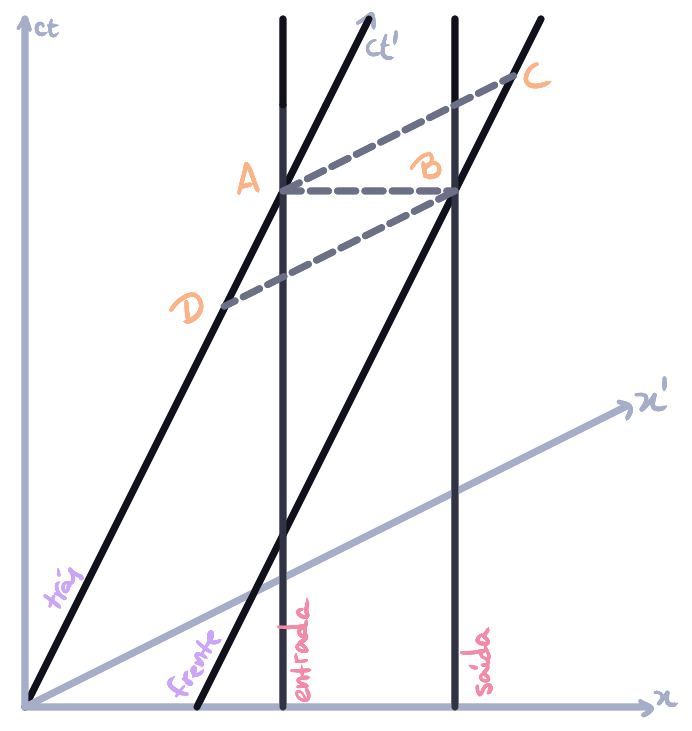
\includegraphics[width=0.5\textwidth]{tunel_trem.png}
    \caption{Diagrama de espaço-tempo}
\end{figure}

\section*{Exercício 6}
Seja \(\Sigma\) o referencial em que \(A\) se move com velocidade \(v_A^C=\frac45c\) e \(B\) se move com velocidade \(v_B^C = \frac35c\) na mesma direção. Neste referencial, a velocidade relativa entre \(A\) e \(B\) é \(v = \frac15c\), de modo que o tempo que \(A\) leva para ultrapassar \(B\) é
\begin{equation*}
    \Delta t = \frac{L_A + L_B}{v},
\end{equation*}
em que \(L_A\) é o comprimento de \(A\) e \(L_B\) de \(B\) neste referencial. Assim,
\begin{equation*}
    \Delta t = \frac{\frac{1}{\gamma_A} + \frac{1}{\gamma_B}}{v}L = \frac{7L}{c}.
\end{equation*}
\section*{Exercício 7}
No referencial \(\Sigma'\) de repouso da barra, suas extremidades se encontram em todo instante no plano \(x_0y_0\) na origem e no ponto \((L_0 \cos\theta_0, L_0 \sin \theta_0)\).

O referencial \(\Sigma'\) se move em relação ao referencial \(\Sigma\) com velocidade \(v\hat{x}\). Pela contração de Lorentz, as extremidades da barra se encontram nas posições \(\left(vt,0\right)\) e \(\left(vt + \frac{L_0\cos\theta_0}{\gamma}, L_0\sin\theta_0\right)\) em um dado instante \(t\). Assim, o comprimento da barra neste referencial é
\begin{equation*}
    L = \sqrt{L_0^2\sin^2\theta_0 + \frac{L_0^2\cos^2\theta_0}{\gamma^2}} = \frac{L_0}{\gamma} \sqrt{\gamma^2\sin^2\theta_0 + \cos^2\theta_0}
\end{equation*}
e o ângulo \(\theta\) que a barra faz com o eixo \(x\) é dado por
\begin{equation*}
    \tan \theta = \gamma \tan \theta_0.
\end{equation*}

\section*{Exercício 8}

\begin{proposition}{\textit{Boost} de um 4-vetor arbitrário}{boost}
    Um quadrivetor \(S^\mu = (\sigma, \vec{s})\) no referencial \(\Sigma\) tem componentes \(S^{\mu'} = (\sigma', \vec{s'})\) no referencial \(\Sigma'\), que se move com velocidade \(\vec{v} = v\hat{n}\) em relação a \(\Sigma\), onde
    \begin{equation*}
        \sigma' = \gamma (\sigma - \beta \vec{s} \cdot \hat{n})
    \end{equation*}
    e
    \begin{equation*}
        \vec{s'} = \vec{s} + \left[(\gamma - 1)(\vec{s} \cdot \hat{n}) - \gamma \beta \sigma\right]\hat{n},
    \end{equation*}
    em que \(\beta = \frac{v}{c}\) e \(\gamma = (1 - \beta^2)^{-\frac12}\).
\end{proposition}
\begin{proof}
    Podemos assumir sem perda de generalidade que \(\hat{n} = \hat{x}\), em que \(\vec{s} = s_x \hat{x} + s_y \hat{y} + s_z \hat{z}\), portanto
    \begin{equation*}
        \left\{
        \begin{aligned}
            \sigma' &= \gamma (\sigma - \beta s_x)\\
            s_x' &= \gamma (s_x - \beta \sigma)\\
            s_y' &= s_y\\
            s_z' &= s_z
        \end{aligned}
        \right.
    \end{equation*}
    são as transformações de Lorentz usuais. Notando que \(s_x = \vec{s}\cdot\hat{n}\), segue que
    \begin{equation*}
        \sigma' = \gamma (\sigma - \beta \vec{s} \cdot\hat{n})\text{ e }s_x' = \gamma (\vec{s} \cdot \hat{n} - \beta \sigma).
    \end{equation*}
    Ainda, \(\vec{s'} = s_x' \hat{x} + s_y' \hat{y} + s_z'\hat{z}\), portanto
    \begin{align*}
        \vec{s'} &= \left(s_x' - s_x\right) \hat{x} + \left(s_x \hat{x} + s_y \hat{y} + s_z \hat{z}\right)\\
                 &= \vec{s} + \left(s_x' - s_x\right) \hat{n}\\
                 &= \vec{s} + \left[\gamma (\vec{s} \cdot \hat{n} - \beta \sigma) - \vec{s}\cdot\hat{n}\right]\hat{n}\\
                 &= \vec{s} + \left[(\gamma - 1)(\vec{s}\cdot\hat{n}) - \gamma \beta \sigma\right]\hat{n},
    \end{align*}
    como desejado.
\end{proof}

No referencial \(\Sigma\), a partícula se move com velocidade \(\vec{u} = u \cos \theta \hat{x} + u \sin \theta \hat{y}\), portanto sua 4-velocidade tem componentes \((\gamma_u c, \gamma_u \vec{u})\) neste referencial. O referencial \(\Sigma'\) se move com velocidade \(\vec{v} = -v\hat{x}\) em relação a \(\Sigma\), de modo que a 4-velocidade da partícula em \(\Sigma'\) tem componentes \((\gamma_w c, \gamma_w \vec{w})\), dadas pela expressão da \cref{prop:boost}, isto é
\begin{align*}
    \gamma_w c &= \gamma_v (\gamma_u c - \beta_v \gamma_u \vec{u} \cdot (-\hat{x}))\\
               &= \gamma_v(\gamma_u c + \beta_v \gamma_u u \cos\theta)\\
               &= \gamma_u \gamma_v (1 + \beta_u \beta_v \cos\theta) c
\end{align*}
e
\begin{align*}
    \gamma_w \vec{w} &= \gamma_u \vec{u} + \left[(\gamma_v - 1)\gamma_u \vec{u} \cdot (-\hat{x}) - \gamma_v \beta_v \gamma_u c\right](-\hat{x})\\
                     &= \gamma_u \vec{u} + \left[(\gamma_v - 1)\gamma_u \beta_u \cos\theta + \gamma_u \gamma_v \beta_v\right]c\hat{x}\\
                     &= \gamma_u \gamma_v \left(\beta_u \cos\theta + \beta_v\right) c\hat{x} + \gamma_u \beta_u \sin \theta c \hat{y}.
\end{align*}
Desse modo,
\begin{equation*}
    \vec{w} = \frac{\beta_u \cos\theta + \beta_v}{1 + \beta_u \beta_v \cos\theta} c \hat{x} + \frac{\beta_u \sin \theta}{\gamma_v \left(1 + \beta_u \beta_v \cos \theta\right)} c \hat{y}
\end{equation*}
é a velocidade da partícula em \(\Sigma'\), que faz um ângulo \(\theta'\) dado por
\begin{equation*}
    \tan \theta' = \frac{\beta_u \sin\theta}{\gamma_v \left(\beta_u \cos\theta + \beta_v\right)},
\end{equation*}
em relação ao eixo \(x\).

Um triângulo retângulo de catetos de comprimento \(L_x\) e \(L_y\) situados ao longo dos eixos \(x\) e \(y\), respectivamente, que se encontra em repouso em \(\Sigma\) é visto por \(\Sigma'\) como um triângulo retângulo de catetos \(L_x'\) e \(L_y'\) que se move com velocidade \(v\hat{x}\). Pelas transformações de Lorentz, obtemos \(L_y' = L_y\) e \(L_x' = \frac{L_x}{\gamma_v}\). Assim, se \(\varphi\) é o ângulo compreendido entre o lado de comprimento \(L_x\) e a hipotenusa no referencial \(\Sigma\), o ângulo \(\varphi'\) análogamente medido em \(\Sigma'\) é dado por
\begin{equation*}
    \tan \varphi' = \gamma_v \tan \varphi.
\end{equation*}

\section*{Exercício 9}
Em um referencial \(S\) em que a 4-posição de uma partícula tem componentes \(x^\mu\), definimos sua 4-velocidade e 4-aceleração pelas componentes
\begin{equation*}
    v^\mu = \diff{x^\mu}{\tau} \text{ e } a^\mu = \diff{v^\mu}{\tau}.
\end{equation*}
Assim, temos \(v^\mu = (\gamma_v c, \gamma_v \vec{v})\), em que \(\vec{v}\) é a 3-velocidade da partícula e \(\gamma_v = \diff{t}{\tau}\), e
\begin{align*}
    a^\mu &= \left(c\diff{\gamma_v}{\tau}, \diff{\gamma_v}{\tau} \vec{v} + \gamma_v \diff{\vec{v}}{\tau}\right)\\
          &= \left(c \gamma_v \dot \gamma_v, \gamma_v \dot \gamma_v \vec{v} + \gamma_v^2 \vec{a} \right),
\end{align*}
onde \(\dot \gamma_v = \diff{\gamma_v}{t}\) e \(\vec{a} = \diff{\vec{v}}{t}\).

Sendo \(\eta\) a métrica de Minkowski, temos
\begin{equation*}
    \eta_{\mu \nu} v^\mu v^\nu = c^2.
\end{equation*}
Derivando em relação a \(\tau\), obtemos
\begin{equation*}
    \eta_{\mu\nu}\diff{v^\mu}{\tau}v^\nu = 0 \implies a^\mu v_\mu  = 0,
\end{equation*}
como desejado.

Em um dado instante em que a velocidade espacial da partícula é \(\vec{u} = u \hat{n}\) no referencial \(S\), tomamos nossa atenção ao referencial \(S'\) que se move em relação a \(S\) com velocidade espacial \(\vec{u}\). Neste mesmo instante, a 4-velocidade da partícula é \(v^{\mu'} = (c, 0)\) no referencial \(S'\), de modo que a componente temporal da 4-aceleração da partícula deve se anular para respeitar a identidade invariante \(a^{\mu'}v_{\mu'} = 0\). Assim,
\begin{equation*}
    a^{\mu'} = (0, \vec{a'})
\end{equation*}
é a 4-aceleração da partícula em \(S'\), em que \(\vec{a'} = \diff{\vec{v}}{t'}\).

\section*{Exercício 10}
Seja \(\Sigma\) o referencial de repouso de uma partícula de massa \(m\). Após seu decaimento em dois fótons de momentos \(\vec{p}_1 \) e \(\vec{p}_2\), temos por conservação de momento que
\begin{equation*}
    \vec{p}_1 = -\vec{p}_2,
\end{equation*}
donde segue que os fótons emitidos têm mesma frequência \(\nu\), mas direções opostas. Assim, neste referencial, a energia da partícula massiva é dada por
\begin{equation*}
    E = 2h\nu,
\end{equation*}
por conservação de energia.

Notemos que  o 4-momento de um dos fótons é dado por
\begin{align*}
    P_1^\mu &= \left(\frac{h \nu}{c}, \frac{h\nu}{c}\hat{n}_1\right)\\
            &= \hbar \left(\frac{\omega}{c}, \vec{k}\right),
\end{align*}
onde \(\omega = 2\pi \nu\) é a frequência angular e \(\vec{k} = \frac{2\pi \nu}{c}\hat{n}_1\) o vetor de onda associados à propagação deste fóton. Deste modo, definimos o 4-vetor de onda \(K^\mu = \frac{1}{\hbar} P^\mu\) para fótons. Após o decaimento, os 4-vetores dos fótons são dados por
\begin{equation*}
    K_1^\mu = \left(\frac{\omega}{c}, \vec{k}\right) \text{ e }K_2^\mu = \left(\frac{\omega}{c}, -\vec{k}\right)
\end{equation*}
no referencial \(\Sigma\).

Seja \(\Sigma'\) o referencial em que a partícula de massa \(m\) se move com velocidade \(\vec{v} = v \hat{n}\). Isto é, o referencial \(\Sigma'\) se move com velocidade \(-\vec{v}\) em relação à \(\Sigma\). Pela \cref{prop:boost}, os 4-vetores de onda dos fótons são dados por
\begin{equation*}
    K_1^{\mu'} = \left(\gamma\frac{\omega + \frac{1}{c} \vec{v} \cdot \vec{k}}{c}, \vec{k} + \left[(\gamma - 1)(\vec{k} \cdot \hat{n}) + \gamma \beta \frac{\omega}{c} \right] \hat{n}\right)
\end{equation*}
e
\begin{equation*}
    K_2^{\mu'} = \left(\gamma\frac{\omega - \frac{1}{c} \vec{v} \cdot \vec{k}}{c}, -\vec{k} + \left[-(\gamma - 1)(\vec{k} \cdot \hat{n}) + \gamma \beta \frac{\omega}{c} \right] \hat{n}\right)
\end{equation*}
em \(\Sigma'\). Assim, o 4-momento da partícula é dado por
\begin{align*}
    P^{\mu'} &= \hbar \left(K_1^{\mu'} + K_2^{\mu'}\right)\\
    &= \left(2\gamma\frac{h\nu}{c}, 2\gamma \beta \frac{h\nu}{c}\hat{n}\right)\\
    &= \left(\gamma \frac{E}{c}, \gamma \beta \frac{E}{c} \hat{n}\right).
\end{align*}

No limite não-relativístico, em que \(\frac{v^2}{c^2} \ll 1\), certamente a diferença entre a energia da partícula no referencial \(\Sigma'\) e no referencial \(\Sigma\) deve tender à energia cinética clássica, isto é,
\begin{equation*}
    \gamma E - E \xrightarrow{\beta^2 \ll 1} \frac12 mv^2.
\end{equation*}
Expandindo \(\gamma - 1\) por séries de Taylor ao redor de \(\beta = 0\), obtemos
\begin{equation*}
    \gamma E - E = E \left[\frac12 \beta^2 + \frac38\beta^4 + O(\beta^6)\right],
\end{equation*}
portanto no limite \(\beta^2 \ll 1\), devemos ter
\begin{equation*}
    \frac12 \beta^2 E = \frac12 m\beta^2c^2 \implies E = mc^2.
\end{equation*}

Deste modo, o momento da partícula no referencial \(\Sigma'\) é dado por \(\vec{p} = \gamma m v \hat{n} = \gamma m \vec{v}\) e sua energia por \(E' = \gamma m c^2\).
\end{document}
